\section{Methodology}
\label{sec:methodology}
The methodology is broken into stages, each answering a different question.
It begins by building the chronological data representation, then tests the
reference models under guarded conditions and validates the teacher-anchored
students. A final set of secondary analyses covers temporal behaviour,
explanation, degraded inputs, calibration, alert burden, and efficiency.
Because each stage plays a different role, their results are not treated as
interchangeable.

\subsection{Datasets and Experimental Design}
\label{subsec:dataset_design}
The experiments used the synthetic Carnegie Mellon University Computer
Emergency Response Team (CERT) r4.2 and r5.2 insider-threat datasets
\cite{GlasserLindauer2013}. Consequently, the findings are interpreted as
controlled benchmark evidence rather than evidence of live organisational
deployment.

\smallskip
CERT r4.2 supported representation development and the initial architecture,
explanation, and degraded-input analyses. It contains 1,000 users,
32,770,222 activity events, 70 insider users, and 7,323 matched malicious
events. Its later chronological partition had already informed development
and is therefore treated as development-evaluation evidence.

\smallskip
The local r5.2 audit identified 2,000 users, 99 insider users, 79,856,699
activity events, and 10,326 unique matched malicious event identifiers
over 517 calendar days from 2 January 2010 to 2 June 2011. The answer
package contained 10,328 records because two identifiers were duplicated.
The calendar was divided globally and chronologically into 413 training
days, 51 validation days, and 53 test days. The resulting sequence
partitions contained 788,000, 64,000, and 68,000 observations, respectively,
with 3,957, 728, and 275 positive sequences.

\smallskip
All 2,000 users occurred in each r5.2 partition. The split therefore
evaluates later behaviour for users represented during training rather than
generalisation to entirely unseen users. Exact sequence identifiers and
user--start-date combinations did not overlap across the chronological
boundaries.

\smallskip
The earlier guarded r5.2 predictive test covered RF, XGBoost,
attention--linear, and frozen-encoder ODST reference families. The final
teacher-anchored students were trained on the r5.2 training partition and
selected using validation evidence only.

\smallskip
Table~\ref{tab:evidence_streams} distinguishes the principal evidence
streams and their permitted interpretations.

\begin{table*}[!t]
\caption{Data Streams and Their Roles}
\label{tab:evidence_streams}
\centering
\footnotesize
\renewcommand{\arraystretch}{1.07}
\setlength{\tabcolsep}{3pt}
\begin{tabularx}{\textwidth}
{@{}>{\raggedright\arraybackslash}p{2.35cm}
>{\raggedright\arraybackslash}p{2.75cm}
Y
Y@{}}
\hline
\textbf{Evidence stream} &
\textbf{Data} &
\textbf{Purpose} &
\textbf{Permitted interpretation} \\
\hline
Development &
CERT r4.2 (train, validation, later) &
Representation, architecture, routing, explanation, degraded-input. &
Development evidence; not an untouched holdout. \\
Guarded reference test &
CERT r5.2 (train, validation, guarded test) &
One-pass RF, XGBoost, attention--linear, frozen-encoder ODST. &
Guarded one-pass evidence for these families only. \\
Teacher-anchored validation &
CERT r5.2 (train, validation) &
End-to-end students, seeds 42, 52, 62. &
Validation-selected reproducibility; not final-student test evidence. \\
Secondary analyses &
Frozen models, predefined partitions &
Same-information, temporal, cohort, explanation, calibration, alert,
latency. &
Bounded by model, seed, partition, and intervention. \\
Post-hoc corroboration &
Previously accessed r5.2 test partition &
Sealed one-pass confirmation of the final students (planned). &
Corroborating only; not an untouched independent test. \\
\hline
\end{tabularx}
\end{table*}

% Replace with the test result once the sealed one-pass confirmation is run.
The r5.2 test partition was used once already, for the reference models.
Running the final teacher-anchored students on it as well would reuse the
same test data, so to keep that result clean we did not do so here. The
final students are evaluated on the r5.2 train/validation protocol instead,
and a sealed one-pass procedure is kept for a later, independent confirmation
on the test partition. No final-student test result is reported in this paper.

\subsection{Chronological Data Preparation}
\label{subsec:data_preparation}
Figure~\ref{fig:data_prep_workflow} summarises the complete chronological
data-preparation pipeline described in this subsection, from the raw
multi-source CERT r4.2 logs through to the two model-input representations
used throughout the study.

\begin{figure}[!t]
\centering
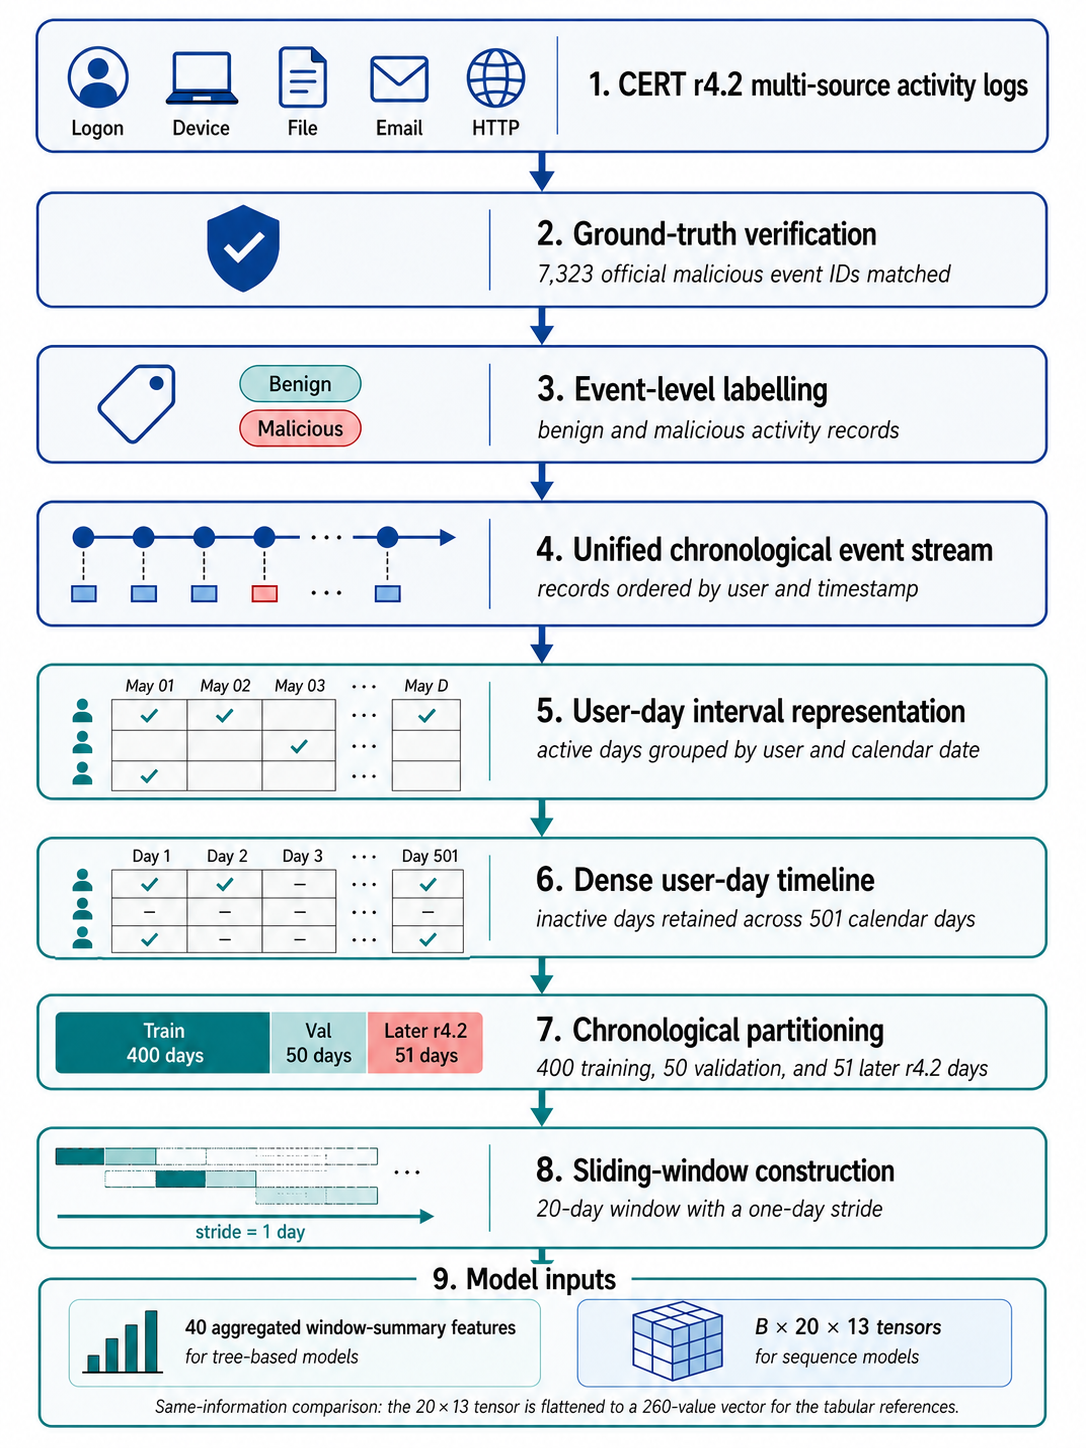
\includegraphics[width=0.85\columnwidth]{figures/data_preparation_workflow.png}
\caption{Chronological data-preparation pipeline, from raw multi-source
CERT r4.2 logs to the two model inputs: 40 window-summary features for the
tree references and \(B\times20\times13\) tensors for the sequence models.}
\label{fig:data_prep_workflow}
\end{figure}

Logon, device, file, email, and HTTP records were converted to a common
event representation and ordered by user and timestamp. Predictive inputs
excluded user identifiers, complete email content, full web addresses,
dates, scenario labels, partition indicators, and answer-derived fields.
Events were aggregated into dense user-day records containing 13 variables:
total event count; logon, device, file, email, and HTTP counts; active
duration; five source-presence indicators; and an active-day indicator.
Inactive days were retained and zero-filled. A user-day was labelled
malicious when it contained at least one verified malicious event.

\smallskip
For an active user-day, duration was
\begin{equation}
\operatorname{duration}_{u,d}
=
\max\!\left[
\operatorname{minutes}
\left(t^{\max}_{u,d}-t^{\min}_{u,d}\right),0
\right],
\label{eq:active_duration}
\end{equation}
where \(t^{\min}_{u,d}\) and \(t^{\max}_{u,d}\) are the earliest and latest
timestamps for user \(u\) on day \(d\).
Twenty-day sequences were constructed with stride one separately inside
each partition, preventing windows from crossing chronological boundaries.
A sequence was positive when any constituent user-day was malicious:
\begin{equation}
\mathbf X_i
=
[\mathbf x_{i,1},\ldots,\mathbf x_{i,20}]
\in\mathbb R^{20\times13}.
\label{eq:input_sequence}
\end{equation}
A custom scaler was fitted only on the training user-days and applied
unchanged to later partitions:
\begin{equation}
x'_{i,f}
=
\frac{x_{i,f}-\mu_f^{\mathrm{train}}}
{\sigma_f^{\mathrm{train}}}.
\label{eq:zscore_scaling}
\end{equation}
The implementation used population standard deviation
(\(\texttt{ddof}=0\)), replaced zero scales by one, standardised all
13 variables including binary indicators, applied no logarithmic
transformation or clipping, and stored the tensors as 32-bit floating-point
values. The r4.2 and r5.2 scalers were fitted independently.

\smallskip
RF and XGBoost references additionally used 40 deterministic window
summaries. In the same-input-content comparison, sequence models received
the \(20\times13\) tensor, whereas flattened models received the same values
in fixed temporal positions as a 260-dimensional vector. This controls
input content while contrasting sequence-aware temporal modelling with
fixed-position flattened representations; it does not isolate chronology
as the only architectural difference.

% =====================================================================
%  C. Teacher-Anchored Sequence--Tree Architecture  (expanded)
% =====================================================================
\subsection{Teacher-Anchored Sequence--Tree Architecture}
\label{subsec:architecture}
Figure~\ref{fig:architecture_pipeline} summarises the forward pipeline.
A time-aware behavioural window is mapped to a single sequence-level
probability in three stages: a bidirectional recurrent encoder that reads
the daily record in both temporal directions, a temporal-attention layer
that compresses the window into one context vector, and a two-layer
oblivious differentiable sparsemax tree (ODST) head that produces the
prediction while exposing its internal routing. This subsection defines
every quantity that later appears in the training objective
(Section~\ref{subsec:teacher_anchoring}).

\begin{figure}[!t]
\centering
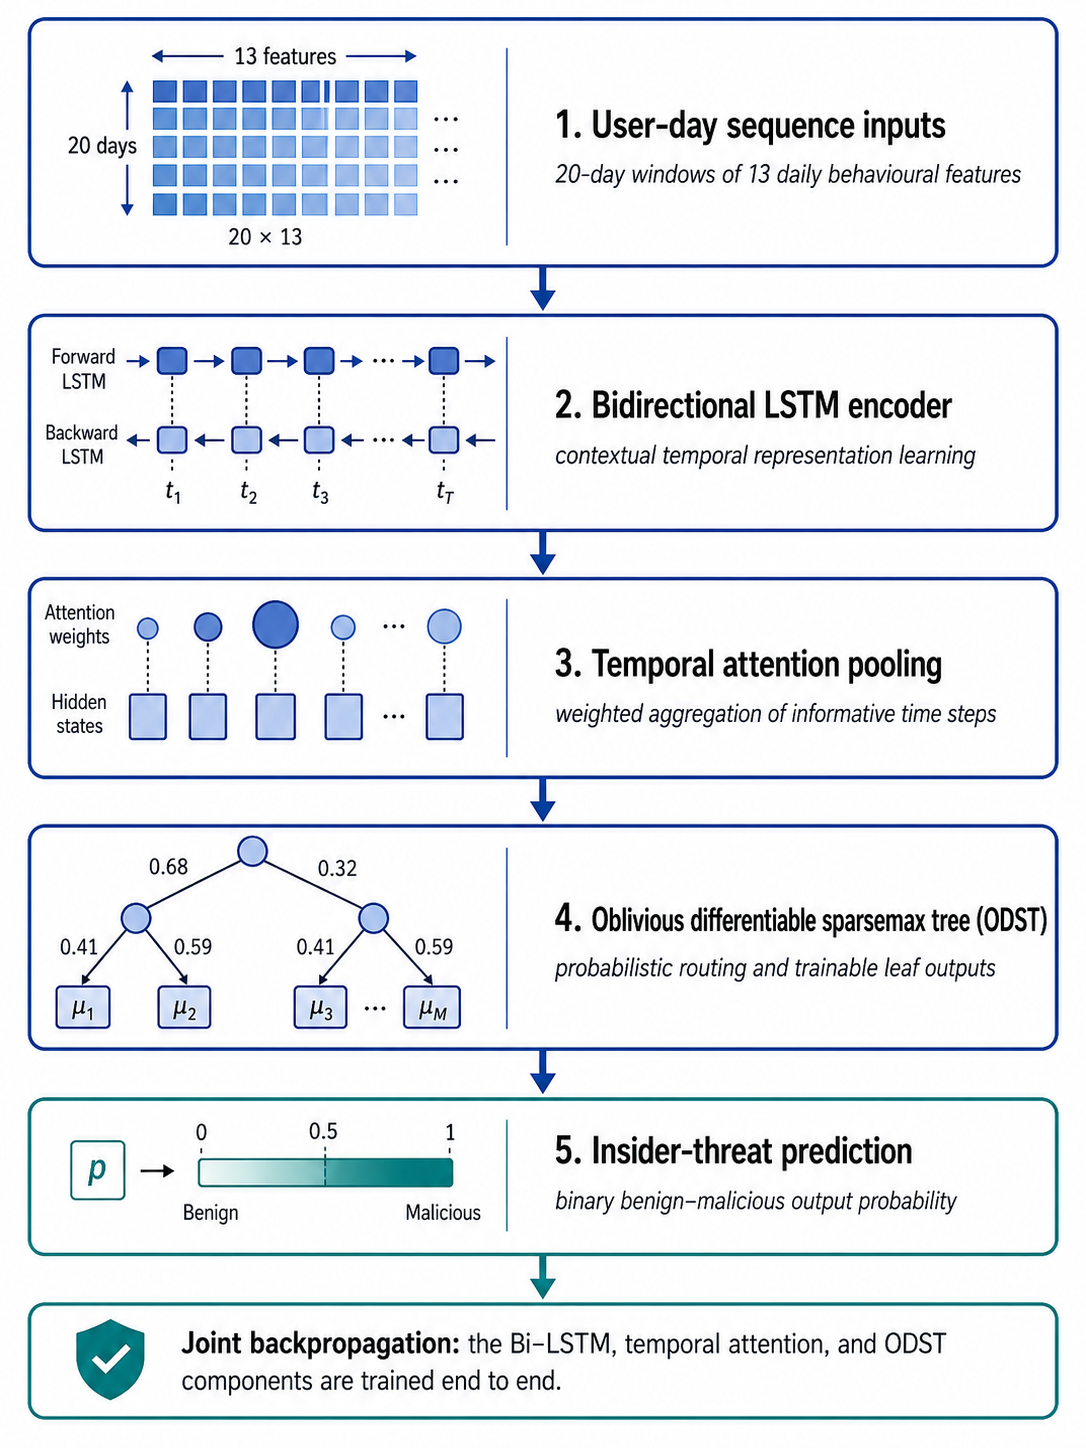
\includegraphics[width=0.85\columnwidth]{figures/architecture_pipeline.png}
\caption{Teacher-anchored sequence--ensemble architecture. A 20-day
behavioural sequence is encoded by a bidirectional LSTM, summarised by
temporal attention into the context vector \(\mathbf z_i\), and classified
by a two-layer ODST head giving \(\hat y_i\in[0,1]\).}
\label{fig:architecture_pipeline}
\end{figure}

\subsubsection{Notation}
\label{subsubsec:notation}
Let \(i\) index one 20-day sequence, \(t\in\{1,\dots,T\}\) a day within the
window with \(T=20\), and \(f\in\{1,\dots,F\}\) a daily behavioural feature
with \(F=13\). The model input is the tensor
\(\mathbf X_i=[\mathbf x_{i,1},\dots,\mathbf x_{i,T}]\in\mathbb R^{T\times F}\),
where \(\mathbf x_{i,t}\in\mathbb R^{F}\) is the standardised feature vector
of day \(t\). The scalar output is the malicious-sequence probability
\(\hat y_i\in[0,1]\).

\subsubsection{Bidirectional recurrent encoder}
\label{subsubsec:encoder}
A single-layer bidirectional long short-term memory (Bi-LSTM) network reads
the window forwards and backwards. At each day \(t\) it produces a
hidden state in each direction, each of size \(H=64\), which are
concatenated:
\begin{equation}
\mathbf h_{i,t}
=
\big[\,\overrightarrow{\mathbf h}_{i,t}\;;\;\overleftarrow{\mathbf h}_{i,t}\,\big]
\in\mathbb R^{2H},
\qquad 2H=128,
\label{eq:bilstm}
\end{equation}
where \(\overrightarrow{\mathbf h}_{i,t}\) and
\(\overleftarrow{\mathbf h}_{i,t}\in\mathbb R^{H}\) are the forward and
backward hidden states and \([\,\cdot\,;\,\cdot\,]\) denotes concatenation.
Reading in both directions lets the representation of day \(t\) depend on
earlier \emph{and} later behaviour in the window. Dropout with probability
\(0.2\) is applied to the sequence of states
\(\{\mathbf h_{i,t}\}_{t=1}^{T}\) before aggregation; the single recurrent
layer has no inter-layer dropout.

\subsubsection{Temporal-attention aggregation}
\label{subsubsec:attention}
The 20 daily states are collapsed into one fixed-size context vector by a
learned attention pooling. Each state is scored, the scores are normalised
across the window by a softmax, and the states are combined by the
resulting weights:
\begin{align}
e_{i,t}
&=
\mathbf v^{\!\top}\tanh\!\big(\mathbf W\,\mathbf h_{i,t}\big),
\label{eq:attn_score}\\[2pt]
\alpha_{i,t}
&=
\frac{\exp(e_{i,t})}{\sum_{t'=1}^{T}\exp(e_{i,t'})},
\qquad
\sum_{t=1}^{T}\alpha_{i,t}=1,
\label{eq:attn_weight}\\[2pt]
\mathbf z_i
&=
\sum_{t=1}^{T}\alpha_{i,t}\,\mathbf h_{i,t}
\in\mathbb R^{2H},
\label{eq:context}
\end{align}
where \(\mathbf W\in\mathbb R^{d_a\times 2H}\) is the attention projection
with hidden size \(d_a=64\), \(\mathbf v\in\mathbb R^{d_a}\) is the scoring
vector, \(e_{i,t}\) is the unnormalised relevance of day \(t\),
\(\alpha_{i,t}\in[0,1]\) is its attention weight, and
\(\mathbf z_i\in\mathbb R^{128}\) is the context vector passed to the tree
head. Intuitively, \(\alpha_{i,t}\) is how much day \(t\) contributes to the
decision, and \(\mathbf z_i\) is the attention-weighted summary of the whole
window.

\subsubsection{Oblivious differentiable sparsemax tree (ODST) head}
\label{subsubsec:odst}
The context vector \(\mathbf z_i\) is classified by a differentiable
soft-tree ensemble. The head contains \(L=2\) stacked layers; each layer
holds \(T_{\mathrm{tree}}=8\) trees of depth \(D=4\), giving
\(M=L\cdot T_{\mathrm{tree}}=16\) trees in total. Two properties distinguish
it from a generic soft decision tree. First, feature selection at every node
uses \emph{sparsemax}, a sparse alternative to softmax that assigns exactly
zero weight to irrelevant features, so each node effectively reads a small
subset of inputs. Softmax was avoided here because it gives every feature a
nonzero weight, so a node would always read all inputs and expose no
selection; sparsemax is what makes the per-node feature choice meaningful and
inspectable. Second, each tree is \emph{oblivious}: all nodes at the
same depth share one split condition, so a tree of depth \(D\) is described
by \(D\) splits rather than \(2^{D}-1\). This is what makes the routing
compact enough to interpret.
\paragraph{Dense two-layer stacking.}
The first layer receives the context vector and emits one scalar per tree,
\(\mathbf O_i^{(1)}\in\mathbb R^{T_{\mathrm{tree}}}=\mathbb R^{8}\). The
second layer receives the context vector \emph{concatenated with} the first
layer's outputs, so its trees can refine on what the first layer already
decided:
\begin{equation}
\mathbf q_i^{(2)}
=
\big[\,\mathbf z_i\;;\;\mathbf O_i^{(1)}\,\big]
\in\mathbb R^{128+8}=\mathbb R^{136}.
\label{eq:stack}
\end{equation}
For uniformity we write \(\mathbf q_i^{(1)}=\mathbf z_i\) for the first
layer, so \(\mathbf q_i^{(\ell)}\) denotes the input to layer \(\ell\).
\paragraph{Soft split at each depth.}
Consider one tree \(m\) in layer \(\ell\). At depth \(k\in\{1,\dots,D\}\) the
node selects features, compares them to a threshold, and outputs a soft
probability of taking the \emph{right} branch:
\begin{align}
\tau_{m,k}
&=
\operatorname{softplus}\!\big(\theta^{\tau}_{m,k}\big)+10^{-4},
\label{eq:temperature}\\[2pt]
p_{i,m,k}
&=
\sigma\!\left(
\frac{\boldsymbol\phi_{m,k}^{\!\top}\mathbf q_i^{(\ell)}-\theta_{m,k}}
{\tau_{m,k}}
\right),
\label{eq:split}
\end{align}
where \(\boldsymbol\phi_{m,k}=\operatorname{sparsemax}(\mathbf f_{m,k})\) is
the sparsemax feature-selection vector obtained from learnable feature
logits \(\mathbf f_{m,k}\) (it picks which inputs the node reads),
\(\theta_{m,k}\) is the learnable split threshold, \(\theta^{\tau}_{m,k}\) is
the raw temperature parameter, \(\tau_{m,k}>0\) is the split temperature
(smaller \(\tau\) gives a sharper, more decisive split; the
\(\operatorname{softplus}(\cdot)+10^{-4}\) keeps it strictly positive), and
\(\sigma(\cdot)\) is the logistic sigmoid. The value \(p_{i,m,k}\in[0,1]\) is
the probability that sample \(i\) is routed right at depth \(k\); the
left-branch probability is \(1-p_{i,m,k}\). A sigmoid is used here precisely
because a split must output a routing probability in \([0,1]\): tanh (range
\(-1\) to \(1\)) or ReLU (unbounded above) could not be read as the
probability of taking a branch, and the complementary form \(1-p_{i,m,k}\)
is only valid when \(p_{i,m,k}\in[0,1]\). Because the tree is oblivious,
this single \(p_{i,m,k}\) is shared by every node at depth \(k\).
\paragraph{From splits to a tree output.}
A leaf of a depth-\(D\) tree corresponds to one root-to-leaf path, encoded as
a binary vector \(\mathbf e=(e_1,\dots,e_D)\in\{0,1\}^{D}\) with \(e_k=1\)
for a right turn and \(e_k=0\) for a left turn at depth \(k\). The
probability that sample \(i\) reaches leaf \(\mathbf e\) of tree \(m\) is the
product of the corresponding branch probabilities:
\begin{equation}
\mu_{i,m,\mathbf e}
=
\prod_{k=1}^{D}
p_{i,m,k}^{\,e_k}\,
\big(1-p_{i,m,k}\big)^{1-e_k},
\qquad
\sum_{\mathbf e}\mu_{i,m,\mathbf e}=1.
\label{eq:leaf_prob}
\end{equation}
Each of the \(2^{D}=16\) leaves carries a trainable scalar response
\(R_{m,\mathbf e}\in\mathbb R\), and the tree's output is the expected leaf
response:
\begin{equation}
o_{i,m}
=
\sum_{\mathbf e\in\{0,1\}^{D}}
\mu_{i,m,\mathbf e}\,R_{m,\mathbf e}.
\label{eq:tree_out}
\end{equation}
Here \(\mu_{i,m,\mathbf e}\in[0,1]\) is the soft membership of sample \(i\)
in leaf \(\mathbf e\) (a "soft" routing because it is a probability, not a
hard 0/1 assignment) and \(R_{m,\mathbf e}\) is the value that leaf
contributes. Equations~\eqref{eq:split}--\eqref{eq:tree_out} are the
differentiable analogue of "follow the branches to a leaf and read its
value," made smooth so the whole head can be trained by gradient descent.
\paragraph{Ensemble readout.}
The raw sequence logit is the mean of all \(M=16\) tree outputs, and the
prediction is its sigmoid:
\begin{equation}
z_i \;=\; \frac{1}{M}\sum_{m=1}^{M} o_{i,m},
\qquad
\hat y_i \;=\; \sigma(z_i).
\label{eq:readout}
\end{equation}
No additional linear or multilayer classification head follows the average;
the prediction is exactly this tree-average, which is what allows each
tree's contribution to the logit to be read off directly
(Section~\ref{subsec:explanation_method}). Figure~\ref{fig:odst_routing}
illustrates Equations~\eqref{eq:split}--\eqref{eq:readout} for a single
oblivious tree.
The complete \(\texttt{node\_head}\) contained 8{,}977 parameters
(feature logits, thresholds, temperatures, and leaf responses across the two
layers, plus a retained but unused linear head kept only for checkpoint
compatibility), of which 8{,}832 participated in the tree-average forward
computation of Equation~\eqref{eq:readout}.

\begin{figure}[!t]
\centering
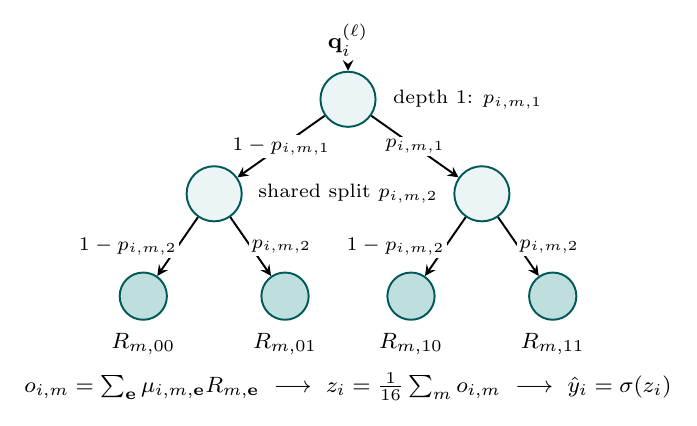
\includegraphics[width=\columnwidth]{figures/odst_routing.png}
\caption{Soft routing of one oblivious tree (drawn at depth two; the model
uses depth four). Each shared split sends sample \(i\) right with
probability \(p_{i,m,k}\) (Eq.~\eqref{eq:split}); leaf-reaching
probabilities multiply along the path (Eq.~\eqref{eq:leaf_prob}), and the
tree output is the probability-weighted sum of the leaf responses
(Eq.~\eqref{eq:tree_out}).}
\label{fig:odst_routing}
\end{figure}

% =====================================================================
%  D. Teacher-Anchored Optimisation  (expanded)
% =====================================================================
\subsection{Teacher-Anchored Optimisation}
\label{subsec:teacher_anchoring}
Training a differentiable tree head jointly with a recurrent encoder is
unstable: the trees can collapse onto a few routes while the encoder drifts.
Teacher anchoring stabilises this by first freezing a fully trained,
identical-architecture \emph{teacher}, then training a \emph{student} whose
prediction logits and routing probabilities are softly pulled toward the
teacher's. For each seed the student is initialised from the corresponding
frozen r5.2 teacher. The teacher is placed in evaluation mode, excluded from
the optimiser, and evaluated without gradient tracking; its logits and route
probabilities are \emph{detached} (treated as fixed targets). The student's
Bi-LSTM, attention block, and ODST head all remain trainable, and the
teacher is discarded after training so inference uses the student alone
(Figure~\ref{fig:teacher_anchored_architecture}).

\begin{figure}[!t]
\centering
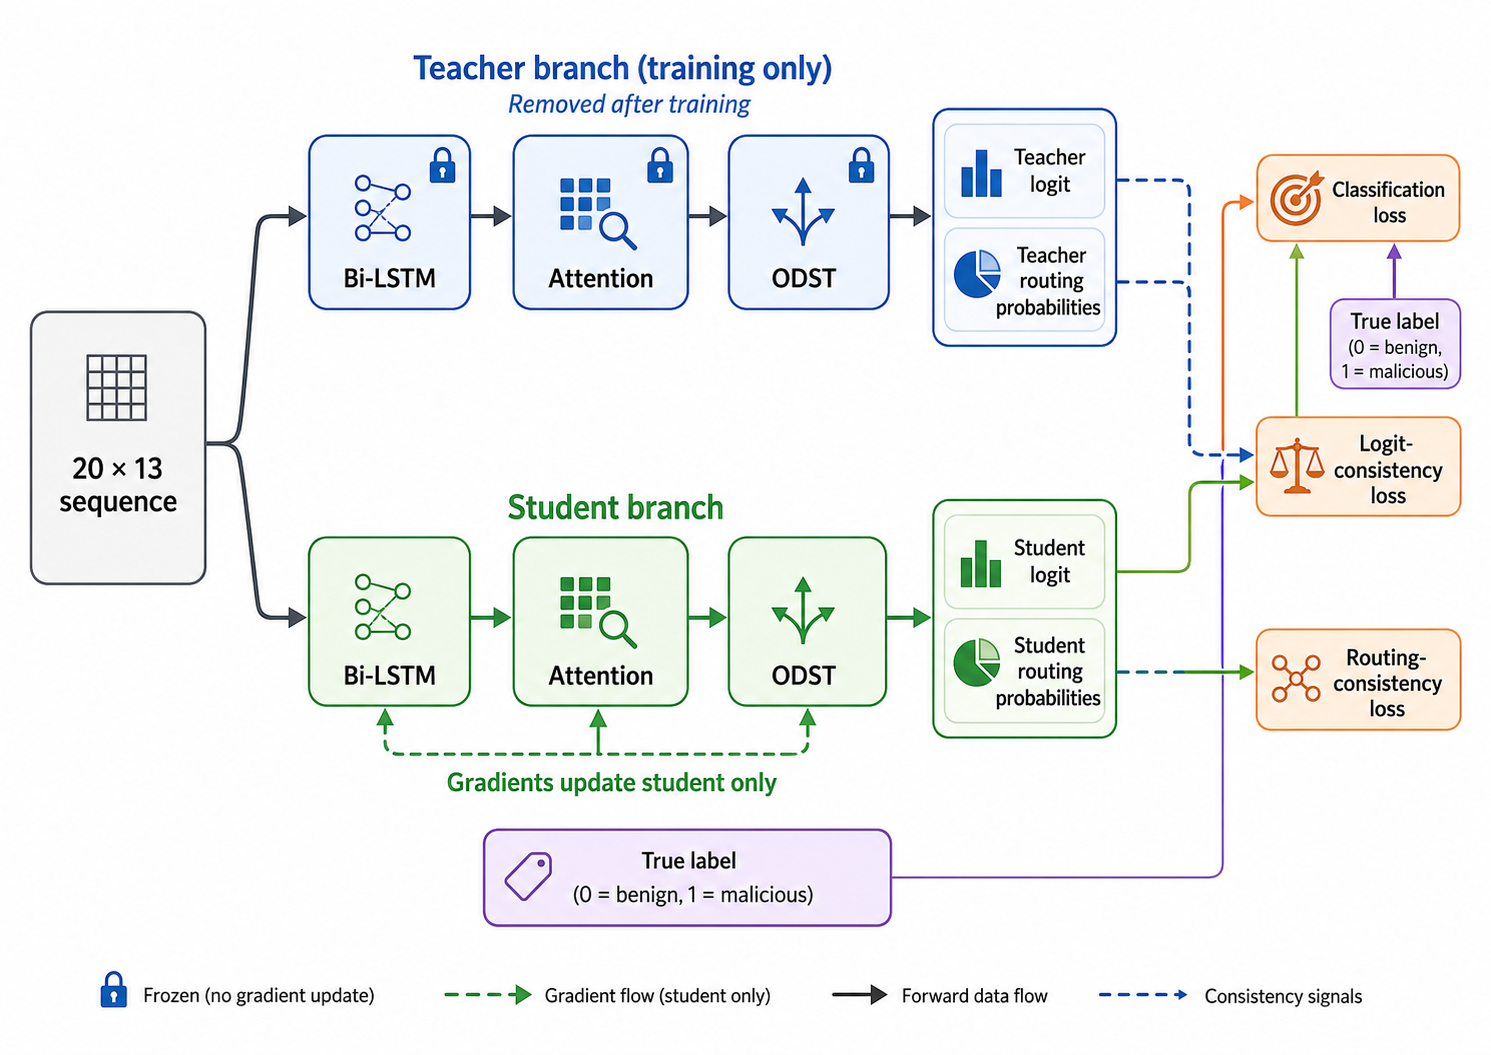
\includegraphics[width=\columnwidth]{figures/fig_teacher_anchored_training_architecture.png}
\caption{Teacher-anchored training. The frozen teacher and trainable
student share the same Bi-LSTM--attention--ODST structure. Detached teacher
logits and routing probabilities anchor the student's consistency losses;
only the student is updated, and inference uses the student alone.}
\label{fig:teacher_anchored_architecture}
\end{figure}

The total training objective is a weighted sum of a classification loss and
two anchoring losses:
\begin{equation}
\mathcal L_{\mathrm{total}}
=
\mathcal L_{\mathrm{cls}}
+\lambda_{\mathrm{logit}}\,\mathcal L_{\mathrm{logit}}
+\lambda_{\mathrm{route}}\,\mathcal L_{\mathrm{route}},
\label{eq:teacher_anchored_loss}
\end{equation}
with fixed anchoring weights
\(\lambda_{\mathrm{logit}}=\lambda_{\mathrm{route}}=0.5\). The weight \(0.5\)
was fixed in advance and not tuned on results; it lets the anchoring guide
the student without overriding the supervised signal.
\paragraph{Classification loss.}
The supervised term is a class-weighted binary cross-entropy computed over a
training batch of \(B\) sequences:
\begin{equation}
\mathcal L_{\mathrm{cls}}
=
-\frac{1}{B}\sum_{i=1}^{B}
\Big[
w_{+}\,y_i\log\sigma(z_i^{S})
+(1-y_i)\log\!\big(1-\sigma(z_i^{S})\big)
\Big],
\label{eq:wbce}
\end{equation}
where \(B\) is the batch size, \(y_i\in\{0,1\}\) is the true label (1 =
malicious), \(z_i^{S}\) is the student logit from
Equation~\eqref{eq:readout}, \(\sigma(z_i^{S})=\hat y_i\) is the predicted
probability, and \(w_{+}\) is the positive-class weight. Because malicious
sequences are rare, \(w_{+}\) makes an error on a positive example cost more
than an error on a negative one. It is set to a fixed fraction of the inverse class-frequency ratio for the r5.2 training partition:
\begin{equation}
w_{+}
=
0.25\cdot\frac{n_{-}}{n_{+}}
=
0.25\cdot\frac{784{,}043}{3{,}957}
=
49.535191,
\label{eq:posweight}
\end{equation}
where \(n_{+}=3{,}957\) is the number of malicious training sequences and
\(n_{-}=784{,}043\) the number of benign ones (of \(788{,}000\) in total).
The ratio \(n_{-}/n_{+}\approx198.14\) is the weight that would make the two
classes contribute equally to the loss; the multiplier \(0.25\) applies a
quarter of that full rebalancing, which up-weights the rare class strongly
enough to be learned while avoiding the precision collapse that full
inverse-frequency weighting tends to cause.
\paragraph{Logit-anchoring loss.}
The first anchoring term keeps the student logit close to the teacher logit,
normalised by the spread of the teacher logits so the penalty is
scale-invariant:
\begin{equation}
\mathcal L_{\mathrm{logit}}
=
\frac{\operatorname{mean}_i\big[(z_i^{S}-\operatorname{sg}(z_i^{T}))^{2}\big]}
{\operatorname{Var}_{\mathrm{pop}}\!\big[\operatorname{sg}(z^{T})\big]+10^{-6}},
\label{eq:logit_anchor}
\end{equation}
where \(z_i^{S}\) and \(z_i^{T}\) are the student and teacher logits for
sample \(i\), \(\operatorname{sg}(\cdot)\) is the stop-gradient operator
(the teacher is a constant target, so no gradient flows into it),
\(\operatorname{mean}_i[\cdot]\) averages the squared difference over the
batch, and \(\operatorname{Var}_{\mathrm{pop}}[\cdot]\) is the population
variance of the teacher logits over the batch. Dividing by this variance
(with \(10^{-6}\) preventing division by zero) means the penalty measures
how far the student is from the teacher \emph{relative} to how spread out
the teacher's scores are, so it neither explodes nor vanishes when logits
are large or small.
\paragraph{Route-anchoring loss.}
The second anchoring term keeps the student's tree routing aligned with the
teacher's. Each ODST layer produces soft right-branch probabilities of shape
\((B,T_{\mathrm{tree}},D)=(B,8,4)\); concatenating the two layers gives the
per-sample route tensors
\(\mathbf P^{S},\mathbf P^{T}\in\mathbb R^{B\times16\times4}\), whose entries
are the \(p_{i,m,k}\) of Equation~\eqref{eq:split} for the student and
teacher respectively. The loss is the elementwise Bernoulli
Kullback--Leibler divergence between them, averaged over all entries:
\begin{equation}
\begin{split}
\mathcal L_{\mathrm{route}}
=\operatorname{mean}\Big[\,
& P^{T}\log\tfrac{P^{T}+\varepsilon}{P^{S}+\varepsilon}\\
&{}+(1-P^{T})\log\tfrac{1-P^{T}+\varepsilon}{1-P^{S}+\varepsilon}\,\Big],
\end{split}
\label{eq:route_anchor}
\end{equation}
where \(P^{S}\) and \(P^{T}\) denote corresponding student and teacher
right-branch probabilities (the teacher tensor is detached), the two terms
are the divergence for the right and left branch of each node, the mean is
taken over all \(B\times16\times4\) entries, and \(\varepsilon=10^{-6}\) guards the
logarithms. Treating each split as a Bernoulli variable, this term
penalises the student for routing samples differently from the teacher, so
the student inherits not just the teacher's scores but its internal
decision paths.

\smallskip
Because the two anchoring terms were always applied together, the combined
anchoring is evaluated as a whole; separate logit-only and route-only
ablations were not performed. The saved student supported
teacher-independent inference.

\subsection{Training and Evaluation}
\label{subsec:training}
The final students used the Adam optimiser with batch size 1,024, encoder and attention
learning rates of \(3\times10^{-5}\), an ODST learning rate of
\(3\times10^{-4}\), zero weight decay, a 15-epoch limit, patience four on
validation average precision, and gradient clipping at norm 1.0. No
scheduler or mixed-precision training was used. Seeds 42, 52, and 62 were
retained, with validation-selected thresholds 0.56, 0.85, and 0.55.
Table~\ref{tab:training_hyperparameters} summarises this configuration.

\begin{table}[!tbp]
\caption{Teacher-Anchored Student Training Configuration}
\label{tab:training_hyperparameters}
\centering
\footnotesize
\renewcommand{\arraystretch}{1.08}
\setlength{\tabcolsep}{2pt}
\begin{tabular*}{\columnwidth}
{@{\extracolsep{\fill}}lr@{}}
\hline
\textbf{Hyperparameter} & \textbf{Value} \\
\hline
Optimiser & Adam \\
Batch size & 1,024 \\
Encoder / attention learning rate & \(3\times10^{-5}\) \\
ODST learning rate & \(3\times10^{-4}\) \\
Weight decay & 0 \\
Epoch limit & 15 \\
Early-stopping patience (validation AP) & 4 \\
Gradient-clipping norm & 1.0 \\
Scheduler / mixed precision & None \\
Retained seeds & 42, 52, 62 \\
Validation-selected thresholds (seeds 42/52/62) & 0.56, 0.85, 0.55 \\
\hline
\end{tabular*}
\end{table}

Predictive viability required student-minus-teacher differences of at least
\(-0.020\) for average precision and \(-0.030\) for F1, together with
representation and routing checks. All three r5.2 seeds passed the recorded
validation gates. These margins were predefined for the r5.2 transfer but
are not described as prospectively preregistered for the earlier r4.2
development.

\smallskip
Average precision, reported as PR-AUC, was the primary ranking measure.
Thresholded predictions used \(p_i\geq\vartheta\). Precision, recall, and
F1 used \(\texttt{zero\_division}=0\). Same-input uncertainty used a paired
user-cluster bootstrap with 2,000 valid resamples and percentile 95\%
intervals. Five predefined comparisons were retained; Bonferroni-adjusted
intervals were sensitivity analyses rather than primary decision rules.

\subsubsection{Evaluation Metrics}
\label{subsubsec:evaluation_metrics}
Let \(TP\), \(TN\), \(FP\), and \(FN\) denote true positives, true
negatives, false positives, and false negatives. Threshold-specific
measures were
\begin{subequations}\label{eq:classification_metrics}
\begin{align}
\mathrm{Precision}
&=
\frac{TP}{TP+FP},
&
\mathrm{Recall}
&=
\frac{TP}{TP+FN},
\\
\mathrm{F1}
&=
2
\frac{\mathrm{Precision}\,\mathrm{Recall}}
{\mathrm{Precision}+\mathrm{Recall}},
&
\mathrm{FPR}
&=
\frac{FP}{FP+TN},
\\
\mathrm{FNR}
&=
\frac{FN}{FN+TP}.
\end{align}
\end{subequations}
Probability quality was summarised using
\begin{subequations}\label{eq:calibration_metrics}
\begin{align}
\mathrm{Brier}
&=
\frac{1}{N}
\sum_{i=1}^{N}
(\widehat y_i-y_i)^2,
\\
\mathrm{LogLoss}
&=
-\frac{1}{N}
\sum_{i=1}^{N}
\left[
y_i\log\widehat y_i
+
(1-y_i)\log(1-\widehat y_i)
\right].
\end{align}
\end{subequations}
For metric \(q\), the three-seed mean and sample standard deviation were
\begin{subequations}\label{eq:seed_summary}
\begin{align}
\overline q
&=
\frac{1}{K}\sum_{k=1}^{K}q_k,
\\
s_q
&=
\sqrt{
\frac{
\sum_{k=1}^{K}(q_k-\overline q)^2
}{
K-1
}
}.
\end{align}
\end{subequations}
All interpretation remained at the sequence or explicitly defined
analytical-unit level. Findings from synthetic CERT benchmarks were not
presented as deployment readiness or direct evidence about real employees.

\subsection{Temporal and Multi-Day Analyses}
\label{subsec:temporal_value_method}
The secondary seed-42 temporal analysis evaluated chronological, reversed,
fixed-shuffle, and reduced-history validation inputs without retraining or
threshold adjustment. One global time permutation, generated with seed
2026, was applied to all feature channels; the final day was not protected.
For retained histories of 1, 5, and 10 days, earlier timesteps were replaced
with feature-wise medians from the scaled training tensor, and the complete
model, including attention, was forwarded again.

\smallskip
A separate r5.2 validation cohort defined a multi-day proxy as a 20-day
window containing malicious activity on at least two distinct calendar
days. The positive subgroup contained 613 overlapping sequence windows
from 26 users and 26 CERT answer-file incidents. Cohort G combined these
windows with all 63,272 benign validation sequences
(\(n=63,885\)). Sequence recall was calculated over the 613 positive
windows using each model's locked validation threshold, while cohort
ranking used average precision. Because stride-one windows generated an
average of approximately 23.6 windows per answer-file incident, these
observations are not interpreted as independent attacks. Incident- and
user-cluster bootstrap procedures were used for positive-subgroup and
cohort comparisons, respectively.

\subsection{Explanation, Calibration, and Alert Analysis}
\label{subsec:explanation_method}
The expanded explanation cohort contained 484 r5.2 validation sequences
from 151 users. Attention faithfulness ranked timesteps by attention weight,
intervened at \(k\in\{1,3,5,10\}\), and compared each top-\(k\) result with
25 matched random-position interventions. Each intervention replaced the
complete 13-feature timestep vector with zero in model-input space and
recomputed attention. These analyses assess model-relative decision
faithfulness and are not causal explanations of employee behaviour.

\smallskip
For the primary ODST analysis, the reference-centred contribution of tree
\(m\) was
\begin{equation}
c_{i,m}
=
\frac{
o_{i,m}-\overline{o}^{\,\mathrm{train}}_m
}{16},
\label{eq:tree_contribution}
\end{equation}
where \(o_{i,m}\) is the tree output of Equation~\eqref{eq:tree_out} and
\(\overline{o}^{\,\mathrm{train}}_m\) is the mean training output for tree
\(m\). Top-ranked tree responses were replaced by their references and
compared with matched random-tree replacement. Earlier raw-output and
median-reference rankings were retained as sensitivity analyses. The
supported claim concerns reference-centred tree-contribution rankings;
routes and reached leaves remain traceable internal outputs rather than
independently validated attributions.

\smallskip
Probability calibration used five-fold user-grouped out-of-fold temperature
scaling on r5.2 validation logits. Each fold fitted a positive temperature
by minimising log loss and evaluated held-out users. Calibration was
reported using Brier score, log loss, and ten-bin equal-width expected
calibration error. Sequence alerts at frozen thresholds were consolidated
within users: alerts on the same date or one calendar day apart belonged
to the same analytical episode, whereas a gap exceeding one day began a
new episode. These episodes are workload summaries, not verified incidents.

\subsection{Controlled Degraded-Input and Efficiency Analyses}
\label{subsec:degraded_input_method}
For the r4.2 paper analysis, source-channel ablation inverse-transformed the
standardised tensor, set the selected raw count and activity indicator to
zero, recomputed available dependent variables, and reapplied the training
scaler. The r5.2 portability study instead assigned zero directly to
standardised source channels. In that space, zero represents the training
mean on the original scale rather than physical source absence; duration
and the active-day indicator were not reconstructed. The two source
protocols are therefore not treated as directly comparable. The
source-channel ablation results reported in
Section~\ref{sec:experimental_results} were produced by the r5.2
scaled-space protocol.
For standardised continuous feature \(x\), noise sensitivity used
\begin{equation}
\begin{aligned}
s&=\max(|x|,10^{-3}), &
\eta&\sim\mathcal N(0,\ell^{2}),\\
\delta&=\operatorname{clip}(s\eta,-\ell s,\ell s), &
x'&=\max(x+\delta,0),
\end{aligned}
\end{equation}
with \(\ell\in\{0.05,0.10,0.20\}\). Only continuous features 0--6 were
changed; binary indicators were retained. One predefined perturbation
realisation was used per declared seed and level, and clean
validation-selected thresholds were not retuned. Route and leaf agreement
at \(\ell=0.05\) was calculated only for observations whose predicted class
remained unchanged.

\smallskip
Component latency used device-resident inputs, inference mode, explicit
CUDA synchronisation, 50 warm-up iterations, and 300 timed iterations.
The separate eight-tree ablation used 20 warm-up and 100 timed iterations;
its absolute times are therefore not treated as measurements from the same
benchmark protocol. The eight-tree implementation did not improve latency.

\subsection{Implementation and Reproducibility}
\label{subsec:implementation_environment}
The retained environment records include Python 3.11.15, PyTorch
2.12.1+cu130, NumPy 2.4.4, Pandas 3.0.3, and Scikit-learn 1.9.0 on a
Windows-based system. Fixed seeds and recorded checkpoints, thresholds,
hashes, and manifests support seeded repeatability. Bit-exact GPU
determinism across hardware, drivers, and software environments is not
claimed. The r5.2 validation tensor has SHA-256 hash
\texttt{\seqsplit{5ac2e7e8fbd50eb62638cdb8c9d444464e02ff2ea20ba55989c36926dd751a5c}},
independently confirmed against the underlying project files. CERT data
were not redistributed.